\documentclass{assignment}
\ProjectInfos{量子光学}{PHYS6251P}{2015 年}{期末考试}{}{陈稼霖}[https://github.com/Chen-Jialin]{SA21038052}

\begin{document}
\begin{prob}
    V 型三能级原子与两个经典光场作用. 频率为 $\omega_1$ 的经典光场与能级 $\lvert a\rangle$, $\lvert b\rangle$ 耦合, 频率为 $\omega_2$ 的经典光场与能级 $\lvert a\rangle$, $\lvert c\rangle$ 耦合. 系统的哈密顿量为 $H=H_0+H_1$, $H_0=\hbar\omega_a\lvert a\rangle\langle a\rvert+\hbar\omega_b\lvert b\rangle\langle b\rvert+\hbar\omega_c\lvert c\rangle\langle c\rvert$,
    \[
        H_1=\frac{\hbar}{2}(\Omega_{R1}e^{-i\phi_1}e^{-i\omega_1t}\lvert a\rangle\langle b\rvert+\Omega_{R2}e^{-i\phi_2}e^{-i\omega_2t}\lvert a\rangle\langle c\rvert)+\text{H.c.}
    \]
    $\Omega_{R1}e^{-i\phi_1}$ 和 $\Omega_{R2}e^{-i\phi_2}$ 是复拉比频率. 原子的波函数可以写为 $\lvert\Psi\rangle=c_a(t)e^{-i\omega_at}\lvert a\rangle+c_be^{-i\omega_bt}\lvert b\rangle+c_c(t)e^{-i\omega_ct}\lvert c\rangle$. 原子和光场共振, 即: $\omega_a-\omega_b=\omega_1$, $\omega_a-\omega_c=\omega_2$, 通过解薛定谔方程, 可以求得波函数.
    \begin{itemize}
        \item[(1)] 求 $c_a(t)$, $c_b(t)$, $c_c(t)$ 所满足的微分方程;
        \item[(2)] 假设原子的初态为 $\lvert\Psi(0)\rangle=\cos\frac{\theta}{2}\lvert b\rangle+\sin\frac{\theta}{2}\lvert c\rangle$, 求出 $c_a(t)$, $c_b(t)$, $c_c(t)$;
        \item[(3)] 当 $\Omega_{R1}$, $\Omega_{R2}$, $\theta$, $\phi_1$, $\phi_2$ 满足什么条件时, 原子在演化过程中始终处于两个能级态 $\lvert b\rangle$, $\lvert c\rangle$ 的叠加态, 而不被激发到激发态上去. 这种现象叫做相干囚禁 (coherent trapping), 从物理上解释这种现象. (见 M. O. Scully, M. S. Zubairy 的书 《quantum optics》 223-224 页, 世界图书出版公司出版, 中国, 北京)
    \end{itemize}
\end{prob}
\begin{sol}
    \begin{itemize}
        \item[(1)] 在基 $\{\lvert a\rangle,\lvert b\rangle,\lvert c\rangle\}$ 下, 系统哈密顿量的矩阵形式为
        \begin{align}
            H=\begin{bmatrix}
                \hbar\omega_a&\frac{\hbar}{2}\Omega_{R1}e^{-i\phi_1}e^{-i\omega_1t}&\frac{\hbar}{2}\Omega_{R2}e^{-i\phi_2}e^{-i\omega_2t}\\
                \frac{\hbar}{2}\Omega_{R1}e^{i\phi_1}e^{i\omega_1t}&\hbar\omega_b&0\\
                \frac{\hbar}{2}\Omega_{R2}e^{i\phi_2}e^{i\omega_2t}&0&\hbar\omega_c
            \end{bmatrix}.
        \end{align}
        波函数的矢量形式为
        \begin{align}
            \lvert\Psi\rangle=\begin{bmatrix}
                c_a(t)e^{-i\omega_at}\\
                c_b(t)e^{-i\omega_bt}\\
                c_c(t)e^{-i\omega_ct}
            \end{bmatrix}.
        \end{align}
        薛定谔方程
        \begin{align}
            i\hbar\frac{\partial}{\partial t}\lvert\Psi\rangle=H\lvert\Psi\rangle
        \end{align}
        的矩阵形式可表为
        {\small
        \begin{gather}
            i\hbar\frac{\partial}{\partial t}\begin{bmatrix}
                c_a(t)e^{-i\omega_at}\\
                c_b(t)e^{-i\omega_bt}\\
                c_c(t)e^{-i\omega_ct}
            \end{bmatrix}=\begin{bmatrix}
                \hbar\omega_a&\frac{\hbar}{2}\Omega_{R1}e^{-i\phi_1}e^{-i\omega_1t}&\frac{\hbar}{2}\Omega_{R2}e^{-i\phi_2}e^{-i\omega_2t}\\
                \frac{\hbar}{2}\Omega_{R1}e^{i\phi_1}e^{i\omega_1t}&\hbar\omega_b&0\\
                \frac{\hbar}{2}\Omega_{R2}e^{i\phi_2}e^{i\omega_2t}&0&\hbar\omega_c
            \end{bmatrix}\begin{bmatrix}
                c_a(t)e^{-i\omega_at}\\
                c_b(t)e^{-i\omega_bt}\\
                c_c(t)e^{-i\omega_ct}
            \end{bmatrix},\\
            \Longrightarrow i\hbar\begin{bmatrix}
                \dot{c}_a(t)e^{-i\omega_at}-i\omega_ac_a(t)e^{-i\omega_at}\\
                \dot{c}_b(t)e^{-i\omega_bt}-i\omega_bc_b(t)e^{-i\omega_bt}\\
                \dot{c}_c(t)e^{-i\omega_ct}-i\omega_cc_c(t)e^{-i\omega_ct}
            \end{bmatrix}=\begin{bmatrix}
                \hbar\omega_ae^{-i\omega_at}+\frac{\hbar}{2}\Omega_{R1}e^{-i\phi_1}e^{-i\omega_1t}c_b(t)e^{-i\omega_bt}+\frac{\hbar}{2}\Omega_{R2}e^{-i\phi_2}e^{-i\omega_2t}c_c(t)e^{-i\omega_ct}\\
                \frac{\hbar}{2}\Omega_{R1}e^{i\phi_1}e^{i\omega_1t}c_a(t)e^{-i\omega_at}+\hbar\omega_bc_b(t)e^{-i\omega_bt}\\
                \frac{\hbar}{2}\Omega_{R2}e^{i\phi_2}e^{i\omega_2t}c_a(t)e^{-i\omega_at}+\hbar\omega_cc_c(t)e^{-i\omega_ct}
            \end{bmatrix},\\
            \Longrightarrow\begin{bmatrix}
                \dot{c}_a(t)\\
                \dot{c}_b(t)\\
                \dot{c}_c(t)
            \end{bmatrix}=\begin{bmatrix}
                -i\frac{\Omega_{R1}}{2}e^{-i\phi_1}c_b(t)-i\frac{\Omega_{R2}}{2}e^{-i\phi_2}c_c(t)\\
                -i\frac{\Omega_{R1}}{2}e^{i\phi_1}c_a(t)\\
                -i\frac{\Omega_{R2}}{2}e^{i\phi_2}c_a(t)
            \end{bmatrix}
        \end{gather}
        }
        即 $c_a(t)$, $c_b(t)$, $c_c(t)$ 满足微分方程:
        \begin{align}
            \dot{c}_a(t)=&-i\frac{\Omega_{R1}}{2}e^{-i\phi_1}c_b(t)-i\frac{\Omega_{R2}}{2}e^{-i\phi_2}c_c(t),\\
            \dot{c}_b(t)=&-i\frac{\Omega_{R1}}{2}e^{i\phi_1}c_a(t),\\
            \dot{c}_c(t)=&-i\frac{\Omega_{R2}}{2}e^{i\phi_2}c_a(t).
        \end{align}
        \item[(2)] 解上述微分方程组得
        {\footnotesize
        \begin{align}
            c_a(t)=&c_a(0)\cos\left(\sqrt{\Omega_{R1}^2+\Omega_{R2}^2}t\right)-i\frac{\Omega_{R1}e^{-i\phi_1}c_b(0)+\Omega_{R2}e^{-i\phi_2}c_c(0)}{\sqrt{\Omega_{R1}^2+\Omega_{R2}^2}}\sin\left(\sqrt{\Omega_{R1}^2+\Omega_{R2}^2}t\right),\\
            c_b(t)=&-i\frac{\Omega_{R1}}{2\sqrt{\Omega_{R1}^2+\Omega_{R2}^2}}\left\{c_a(0)\sin\left(\sqrt{\Omega_{R1}^2+\Omega_{R2}^2}t\right)+i\frac{\Omega_{R1}e^{-i\phi_1}c_b(0)+\Omega_{R2}e^{-i\phi_2}c_c(0)}{\sqrt{\Omega_{R1}^2+\Omega_{R2}^2}}\left[\cos\left(\sqrt{\Omega_{R1}^2+\Omega_{R2}^2}t\right)-1\right]\right\}+c_b(0),\\
            c_c(t)=&-i\frac{\Omega_{R2}}{2\sqrt{\Omega_{R1}^2+\Omega_{R2}^2}}\left\{c_a(0)\sin\left(\sqrt{\Omega_{R1}^2+\Omega_{R2}^2}t\right)+i\frac{\Omega_{R1}e^{-i\phi_1}c_b(0)+\Omega_{R2}e^{-i\phi_2}c_c(0)}{\sqrt{\Omega_{R1}^2+\Omega_{R2}^2}}\left[\cos\left(\sqrt{\Omega_{R1}^2+\Omega_{R2}^2}t\right)-1\right]\right\}+c_c(0).
        \end{align}
        }
        原子的初态为 $\lvert\Psi(0)\rangle=\cos\frac{\theta}{2}\lvert b\rangle+\sin\frac{\theta}{2}\lvert c\rangle$, 即 $c_a(0)=0$, $c_b(0)=\cos\frac{\theta}{2}$, $c_c(0)=\sin\frac{\theta}{2}$, 故
        \begin{align}
            c_a(t)=&-i\frac{\Omega_{R1}e^{-i\phi_1}\cos\frac{\theta}{2}+\Omega_{R2}e^{-i\phi_2}\sin\frac{\theta}{2}}{\sqrt{\Omega_{R1}^2+\Omega_{R2}^2}}\sin\left(\sqrt{\Omega_{R1}^2+\Omega_{R2}^2}t\right),\\
            c_b(t)=&\frac{\Omega_{R1}^2e^{-i\phi_1}\cos\frac{\theta}{2}+\Omega_{R1}\Omega_{R2}e^{-i\phi_2}\sin\frac{\theta}{2}}{2(\Omega_{R1}^2+\Omega_{R2}^2)}\left[\cos\left(\sqrt{\Omega_{R1}^2+\Omega_{R2}^2}t\right)-1\right]+\cos\frac{\theta}{2},\\
            c_c(t)=&\frac{\Omega_{R1}\Omega_{R2}e^{-i\phi_1}\cos\frac{\theta}{2}+\Omega_{R2}^2e^{-i\phi_2}\sin\frac{\theta}{2}}{2(\Omega_{R1}^2+\Omega_{R2}^2)}\left[\cos\left(\sqrt{\Omega_{R1}^2+\Omega_{R2}^2}t\right)-1\right]+\sin\frac{\theta}{2}.
        \end{align}
        \item[(3)] 当
        \begin{gather}
            c_a(t)=0,\\
            \Longrightarrow\Omega_{R1}e^{-i\phi_1}\cos\frac{\theta}{2}+\Omega_{R2}e^{-i\phi_2}\sin\frac{\theta}{2}=0,\\
            \Longrightarrow\theta=-2\arctan\left[\frac{\Omega_{R1}}{\Omega_{R2}}e^{-i(\phi_1-\phi_2)}\right]
        \end{gather}
        时, 发生相干囚禁, 其物理图像为光场激发下, 由 $\lvert b\rangle$ 向 $\lvert a\rangle$ 跃迁和由 $\lvert c\rangle$ 向 $\lvert a\rangle$ 跃迁产生的 $\lvert a\rangle$ 的概率幅变化抵消.
    \end{itemize}
\end{sol}

\begin{prob}
    增加了一个光子的相干态 (Single-photon-added coherent state (SPACS)), $\lvert\alpha,1\rangle=\frac{a^{\dagger}}{\sqrt{1+\abs{\alpha}^2}}\lvert\alpha\rangle$, 考虑该辐射场的两个厄米算符 $X_1=\frac{1}{2}(a+a^{\dagger})$, $X_2=\frac{1}{2i}(a-a^{\dagger})$, 它们分别对应于场的复振幅的实部和虚部, 满足对易关系 $[X_1,X_2]=\frac{i}{2}$. 当 $\alpha$ 取何值时 (本题 $\alpha$ 取正实数) SPACS 态是压缩态. (提示: 压缩条件 $(\Delta X_1)^2<1/4$ 或 $(\Delta X_2)^2<1/4$).
\end{prob}
\begin{sol}
    $\Delta X_1$ 的涨落计算见 2011 年第 4 题, 当 $\abs{\alpha}>1$ 时, $\Delta X_1<1$, 是压缩态.

    $X_2$ 的均值为
    \begin{align}
        \notag\langle X_2\rangle=&\langle\alpha\rvert\frac{a}{\sqrt{1+\abs{\alpha}^2}}\frac{1}{2i}(a-a^{\dagger})\frac{a^{\dagger}}{\sqrt{1+\abs{\alpha}^2}}\lvert\alpha\rangle\\
        \notag=&\frac{1}{2i(1+\abs{\alpha}^2)}\langle\alpha\rvert a(a-a^{\dagger})a^{\dagger}\lvert\alpha\rangle\\
        \notag=&\frac{1}{2i(1+\abs{\alpha}^2)}\langle\alpha\rvert(aaa^{\dagger}-aa^{\dagger}a^{\dagger})\lvert\alpha\rangle\\
        \notag=&\frac{1}{2i(1+\abs{\alpha}^2)}\langle\alpha\rvert[a(a^{\dagger}a+1)-(a^{\dagger}a+1)a^{\dagger}]\lvert\alpha\rangle\\
        \notag=&\frac{1}{2i(1+\abs{\alpha}^2)}\langle\alpha\rvert(aa^{\dagger}a+a-a^{\dagger}aa^{\dagger}+a^{\dagger})\lvert\alpha\rangle\\
        \notag=&\frac{1}{2i(1+\abs{\alpha}^2)}\langle\alpha\rvert[(a^{\dagger}a+1)a+a-a^{\dagger}(a^{\dagger}a+1)+a^{\dagger}]\lvert\alpha\rangle\\
        \notag=&\frac{1}{2i(1+\abs{\alpha}^2)}\langle\alpha\rvert(a^{\dagger}aa+2a-a^{\dagger}a^{\dagger}a+2a^{\dagger})\lvert\alpha\rangle\\
        \notag=&\frac{1}{2i(1+\abs{\alpha}^2)}\langle\alpha\rvert(\alpha^3+2\alpha-\alpha^3-2\alpha)\lvert\alpha\rangle\\
        =&0.
    \end{align}
    $X_2^2$ 的均值为
    \begin{align}
        \notag\langle X_2^2\rangle=&\langle\alpha\rvert\frac{a}{\sqrt{1+\abs{\alpha}^2}}\left[\frac{1}{2i}(a-a^{\dagger})\right]^2\frac{a^{\dagger}}{\sqrt{1+\abs{\alpha}^2}}\lvert\alpha\rangle\\
        \notag=&-\frac{1}{4(1+\abs{\alpha}^2)}\langle\alpha\rvert a(aa-aa^{\dagger}-a^{\dagger}a+a^{\dagger}a^{\dagger})a^{\dagger}\lvert\alpha\rangle\\
        \notag=&-\frac{1}{4(1+\abs{\alpha}^2)}\langle\alpha\rvert a(aa-2a^{\dagger}a-1+a^{\dagger}a^{\dagger})a^{\dagger}\lvert\alpha\rangle\\
        \notag=&-\frac{1}{4(1+\abs{\alpha}^2)}\langle\alpha\rvert(aaaa^{\dagger}-2aa^{\dagger}aa^{\dagger}-aa^{\dagger}+aa^{\dagger}a^{\dagger}a^{\dagger})\lvert\alpha\rangle\\
        \notag=&-\frac{1}{4(1+\abs{\alpha}^2)}\langle\alpha\rvert[aa(a^{\dagger}a+1)-2(a^{\dagger}a+1)(a^{\dagger}a+1)-(a^{\dagger}a+1)+(a^{\dagger}a+1)a^{\dagger}a^{\dagger}]\lvert\alpha\rangle\\
        \notag=&-\frac{1}{4(1+\abs{\alpha}^2)}\langle\alpha\rvert(aaa^{\dagger}a+aa-2a^{\dagger}aa^{\dagger}a-4a^{\dagger}a-2-a^{\dagger}a-1+a^{\dagger}aa^{\dagger}a^{\dagger}+a^{\dagger}a^{\dagger})\lvert\alpha\rangle\\
        \notag=&-\frac{1}{4(1+\abs{\alpha}^2)}\langle\alpha\rvert[a(a^{\dagger}a+1)a+aa-2a^{\dagger}(a^{\dagger}a+1)a-4a^{\dagger}a-2-a^{\dagger}a-1+a^{\dagger}(a^{\dagger}a+1)a^{\dagger}+a^{\dagger}a^{\dagger}]\lvert\alpha\rangle\\
        \notag=&-\frac{1}{4(1+\abs{\alpha}^2)}\langle\alpha\rvert(aa^{\dagger}aa+2aa-2a^{\dagger}a^{\dagger}aa-2a^{\dagger}a-4a^{\dagger}a-2-a^{\dagger}a-1+a^{\dagger}a^{\dagger}aa^{\dagger}+2a^{\dagger}a^{\dagger})\lvert\alpha\rangle\\
        \notag=&-\frac{1}{4(1+\abs{\alpha}^2)}\langle\alpha\rvert[(a^{\dagger}a+1)aa+2aa-2a^{\dagger}a^{\dagger}aa-2a^{\dagger}a-4a^{\dagger}a-2-a^{\dagger}a-1+a^{\dagger}a^{\dagger}(a^{\dagger}a+1)+2a^{\dagger}a^{\dagger}]\lvert\alpha\rangle\\
        \notag=&-\frac{1}{4(1+\abs{\alpha}^2)}\langle\alpha\rvert(a^{\dagger}aaa+3aa-2a^{\dagger}a^{\dagger}aa-2a^{\dagger}a-4a^{\dagger}a-2-a^{\dagger}a-1+a^{\dagger}a^{\dagger}a^{\dagger}a+3a^{\dagger}a^{\dagger})\lvert\alpha\rangle\\
        \notag=&-\frac{1}{4(1+\abs{\alpha}^2)}\langle\alpha\rvert(\alpha^4+3\alpha^2-2\alpha^4-2\alpha^2-4\alpha^2-2-\alpha^2-1+\alpha^4+3\alpha^2)\lvert\alpha\rangle\\
        \notag=&\frac{\alpha^2+3}{4(1+\alpha^2)}>\frac{1}{4}.
    \end{align}
    $X_2$ 的涨落为
    \begin{align}
        \Delta X_2=\sqrt{\langle X_2^2\rangle-\langle X_2\rangle^2}=\sqrt{\langle X_2^2\rangle}>\frac{1}{2},
    \end{align}
    故无法由 $\Delta X_2$ 判断是否存在压缩.

    综上, 当 $\abs{\alpha}>1$ 时, SPACS 态为压缩态.
\end{sol}

\begin{prob}
    考虑一个理想的光学腔, 腔里有单模辐射场 $\lvert\phi(0)\rangle_F=\frac{1}{\sqrt{2}}(\lvert 0\rangle-i\lvert 10\rangle)$. 处于基态与单模场共振的二能级原子 $\lvert\varphi(0)\rangle_A=\lvert g\rangle$ 进入该光学腔, 与场发生作用, 相互作用的哈密顿量为 $H_I=\hbar g(\sigma_+a^2+\sigma_-(a^{\dagger})^2)$ (在相互作用绘景中研究). 系统的演化方程为 $\lvert\Psi\rangle_{AF}=e^{-\frac{i}{\hbar}H_It}\lvert\phi(0)\rangle_R\lvert\varphi(0)\rangle_A$. 作用一段时间后原子从腔中逸出. 经探测: 出射原子处于激发态 $\lvert e\rangle$.
    \begin{itemize}
        \item[(1)] 计算该单模场初始时刻 $\lvert\phi(0)\rangle_F$ 的平均光子数 $\bar{n}$;
        \item[(2)] 任意时刻系统的态 $\lvert\Psi(t)\rangle_{AF}$;
        \item[(3)] 原子出射后, 腔内的辐射场的平均光子数变为多少?
    \end{itemize}
\end{prob}
\begin{sol}
    \begin{itemize}
        \item[(1)] 该单模场初始时刻的平均光子数为
        \begin{align}
            \bar{n}=_F\langle\phi(0)\rvert a^{\dagger}a\lvert\phi(0)\rangle_F=5.
        \end{align}
        \item[(2)] 设任意时刻系统的态为
        \begin{align}
            \lvert\Psi(t)\rangle_{AF}=\sum_{n=0}^{\infty}[C_{e,n}(t)\lvert e,n\rangle+C_{g,n}(t)\lvert g,n\rangle].
        \end{align}
        将其代入薛定谔方程中得
        \begin{align}
            i\hbar\frac{\partial}{\partial t}\lvert\Psi(t)\rangle_{AF}=H_I\lvert\Psi(t)\rangle_{AF},
        \end{align}
        有
        \begin{align}
            \dot{C}_{e,n}(t)=&-igC_{g,n+2}\sqrt{(n+1)(n+2)},\\
            \dot{C}_{g,n+2}(t)=&-igC_{e,n}\sqrt{(n+1)(n+2)},
        \end{align}
        解得
        \begin{align}
            C_{e,n}(t)=&C_{e,n}(0)\cos[\sqrt{(n+1)(n+2)}gt]-iC_{g,n+2}(0)\sin[\sqrt{(n+1)(n+2)}gt],\\
            C_{g,n+2}(t)=&C_{g,n+2}(0)\cos[\sqrt{(n+1)(n+2)}gt]-iC_{e,n}(0)\sin[\sqrt{(n+1)(n+2)}gt].
        \end{align}
        系统的初始状态为
        \begin{align}
            \lvert\Psi(0)\rangle_{AF}=\lvert\varphi(0)\rangle_A\otimes\lvert\phi(0)\rangle_F=\frac{1}{\sqrt{2}}\lvert g\rangle(\lvert 0\rangle-i\lvert 10\rangle),
        \end{align}
        即 $C_{g,0}=\frac{1}{\sqrt{2}}$, $C_{g,10}=-\frac{i}{\sqrt{2}}$, 故
        \begin{align}
            C_{e,8}=&-\frac{1}{\sqrt{2}}\sin(\sqrt{90}gt),\\
            C_{g,10}=&-\frac{i}{\sqrt{2}}\cos(\sqrt{90}gt),
        \end{align}
        即 $t$ 时刻系统的态为
        \begin{align}
            \lvert\Psi(t)\rangle_{AF}=-\frac{1}{\sqrt{2}}\sin(\sqrt{90}gt)\lvert e,8\rangle-\frac{i}{\sqrt{2}}\cos(\sqrt{90}gt)+\frac{1}{\sqrt{2}}.
        \end{align}
        \item[(3)] 由于探测得出射原子处于激发态 $\lvert e\rangle$, 故系统的态塌缩至 $\lvert 8\rangle$, 此时腔内的辐射场的平均光子数为 $8$.
    \end{itemize}
\end{sol}

\begin{prob}
    由一个赝自旋算符 $S_+=\lvert e\rangle\langle g\rvert$, $S_-=\lvert g\rangle\langle e\rvert$ 和 $S_3=(\lvert e\rangle\langle e\rvert-\lvert g\rangle\langle g\rvert)/2$ 描述的二能级原子, 可定义两个厄米算符: $S_1=(S_++S_-)/2$, $S_2=(S_+-S_-)/(2i)$, 他们的对易关系 $[S_1,S_2]=iS_3$, $S_3=1/2\sigma_z$. 相应的海森堡不确定关系为 $(\Delta S_1)^2(\Delta S_2)^2\geq 1/4\abs{\langle S_3\rangle}^2$, 这里 $(\Delta S_i)^2=\langle S_i^2\rangle-\langle S_i\rangle^2$ 是原子算符 $S_i$ 的量子涨落. 如果量子涨落满足 $(\Delta S_i)^2<1/2\abs{\langle S_3\rangle}$ ($i=1$ 或 $2$), 我们说原子算符的涨落被压缩, 原子出现压缩效应. 当原子处于 $\lvert\Psi\rangle=\cos(\frac{\theta}{2})\lvert e\rangle+\sin(\frac{\theta}{2})\lvert g\rangle$ 时 $S_1$ 的平均值 $\langle S_1\rangle$, 求出分量 $S_1$ 压缩的条件.
\end{prob}
\begin{sol}
    \begin{align}
        S_1=\frac{1}{2}(S_++S_-)=\frac{1}{2}(\lvert e\rangle\langle g\rvert+\lvert g\rangle\langle e\rvert).
    \end{align}
    $S_1$ 的平均值为
    \begin{align}
        \langle S_1\rangle=&\langle\Psi\rvert\frac{1}{2}(\lvert e\rangle\langle g\rvert+\lvert g\rangle\langle e\rvert)\lvert\Psi\rangle=\sin\frac{\theta}{2}\cos\frac{\theta}{2}=\frac{1}{2}\sin\theta.
    \end{align}
    $S_1^2$ 的平均值为
    \begin{align}
        \langle S_1^2\rangle=&\langle\Psi\rvert S_1^2\lvert\Psi\rangle=\frac{1}{4}\langle\Psi\rvert(\lvert e\rangle\langle e\rvert+\lvert g\rangle\langle g\rvert)\lvert\Psi\rangle=\frac{1}{4}.
    \end{align}
    $S_1$ 的涨落为
    \begin{align}
        \Delta S_1=\sqrt{\langle S_1^2\rangle-\langle S_1\rangle^2}=\frac{1}{2}\sqrt{1-\sin^2\theta}.
    \end{align}

    \begin{align}
        \langle S_3\rangle=\langle\Psi\rvert S_3\lvert\Psi\rangle=\frac{1}{2}\left(\cos^2\frac{\theta}{2}-\sin^2\frac{\theta}{2}\right)=\frac{1}{2}\cos\theta.
    \end{align}
    分量 $S_1$ 压缩的条件为
    \begin{gather}
        (\Delta S_1)^2=\frac{1}{4}(1-\sin^2\theta)<\frac{1}{2}\abs{\langle S_3\rangle}=\frac{1}{4}\abs{\cos\theta},\\
        \Longrightarrow\theta\neq n\pi,\quad n=1,2,\cdots.
    \end{gather}
\end{sol}

\begin{prob}
    设原子初态 $\lvert\varphi(0)\rangle_A=\cos\alpha\lvert e\rangle+\sin\alpha\lvert g\rangle$, 光场初态是粒子数态 $\lvert\varphi(0)\rangle_F=\lvert 6\rangle$. 该原子与光场之间的相互作用可用双光子 J-C 模型描述, 在共振条件和相互作用绘景中其哈密顿量表示为 $H_1=\hbar g(\sigma_+a^2+\sigma_-(a^{\dagger})^2)$, 求任意时刻 $t$,
    \begin{itemize}
        \item[(1)] 该复合系统态矢.
        \item[(2)] 原子处于激发态的概率, 画出概率图形 ($\alpha=\pi/4$, 横坐标表示时间, 纵坐标表示概率). (要求给出程序)
    \end{itemize}
\end{prob}
\begin{sol}
    \begin{itemize}
        \item[(1)] 设系统的状态为
        \begin{align}
            \lvert\varphi(t)\rangle_{AF}=\sum_{n=0}^{\infty}[C_{e,n}(t)\lvert e,n\rangle+C_{g,n}\lvert g,n\rangle].
        \end{align}
        相互作用绘景下, 系统的状态演化遵循薛定谔方程:
        \begin{align}
            i\hbar\frac{\partial}{\partial t}\lvert\varphi(t)\rangle_{AF}=H_1\lvert\varphi(t)\rangle_{AF},
        \end{align}
        即
        \begin{align}
            \dot{C}_{e,n}(t)=&-ig\sqrt{(n+1)(n+2)}C_{g,n+2}(t),\\
            \dot{C}_{g,n+2}(t)=&-ig\sqrt{(n+1)(n+2)}C_{e,n}(t),
        \end{align}
        解得
        \begin{align}
            C_{e,n}(t)=&C_{e,n}(0)\cos[\sqrt{(n+1)(n+2)}gt]-iC_{g,n+2}(0)\sin[\sqrt{(n+1)(n+2)}gt],\\
            C_{g,n+2}(t)=&C_{g,n+2}(0)\cos[\sqrt{(n+1)(n+2)}gt]-iC_{e,n}(0)\sin[\sqrt{(n+1)(n+2)}gt].
        \end{align}
        原子初态 $\lvert\varphi(0)\rangle_A=\cos\alpha\lvert e\rangle+\sin\alpha\lvert g\rangle$, 光场初态为粒子数态 $\lvert\varphi(0)\rangle_F=\lvert 6\rangle$, 即 $C_{e,6}=\cos\alpha$, $C_{g,6}=\sin\alpha$, 将其代入上面两式得
        \begin{align}
            C_{e,6}(t)=&\cos\alpha\cos(\sqrt{56}gt),\\
            C_{g,8}(t)=&-i\cos\alpha\sin(\sqrt{56}gt),\\
            C_{g,6}(t)=&\sin\alpha\cos(\sqrt{30}gt),\\
            C_{e,4}(t)=&-i\sin\alpha\cos(\sqrt{30}gt),
        \end{align}
        故任意时刻 $t$ 该复合系统态矢为
        \begin{align}
            \lvert\varphi(t)\rangle_{AF}=-i\cos\alpha\sin(\sqrt{56}gt)+\cos\alpha\cos(\sqrt{56}gt)\lvert e,6\rangle+\sin\alpha\cos(\sqrt{30}gt)-i\sin\alpha\cos(\sqrt{30}gt).
        \end{align}
        \item[(2)] 任意时刻 $t$ 原子处于激发态的概率为
        \begin{align}
            P_e=\abs{C_{e,6}}^2+\abs{C_{e,4}}^2=\cos^2\alpha\cos^2(\sqrt{56}gt)+\sin^2\alpha\cos^2(\sqrt{30}gt).
        \end{align}
        概率图形如图 \ref{2014-5} 所示.
        \begin{figure}[H]
            \centering
            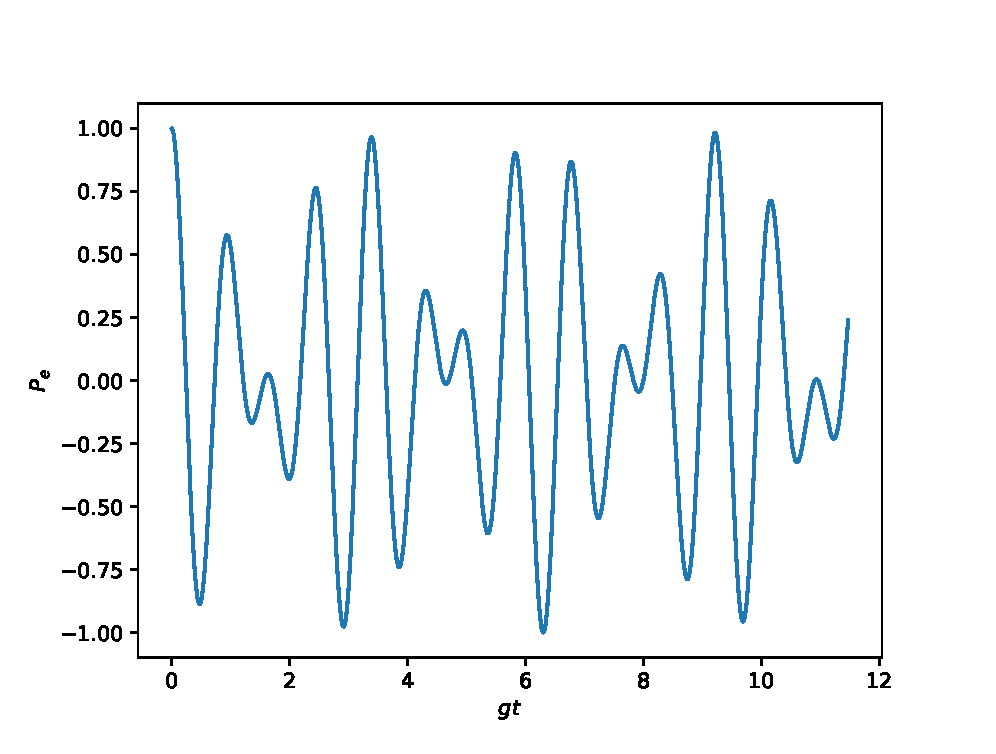
\includegraphics[width=.5\columnwidth]{Figures/2014-5.eps}
            \caption{任意时刻 $t$ 原子处于激发态的概率.}
            \label{2014-5}
        \end{figure}
    \end{itemize}
\end{sol}

\begin{prob}
    一个二能级原子 A 与热库 E (环境) 相互作用如下: $U_{AE}\lvert g\rangle_A\lvert 0\rangle_E=\lvert e\rangle_A\lvert 0\rangle_E$, $U_{AE}\lvert e\rangle_A\lvert 0\rangle_E=\sqrt{1-p}\lvert e\rangle_A\lvert 0\rangle_E+\sqrt{p}\lvert g\rangle_A\lvert 1\rangle_E$, 其中 $p$ 与时间有关, $\lvert 0\rangle_E$ 是环境的真空态. 原子的演化可用 Kraus 算符和表示: $\rho_A(t)=\sum_iM_i\rho_A(0)M_i^{\dagger}$. Kraus 算符的定义是: $M_i=_E\langle i\rvert U_{AE}\lvert 0\rangle_E$.
    \begin{itemize}
        \item[(1)] 试求出 $M_0$ 和 $M_1$.
        \item[(2)] 设原子初态为 $\rho_A(0)=\begin{bmatrix}
            a&b\\
            d&c
        \end{bmatrix}$, 求出 $\rho_A(t)$.
    \end{itemize}
\end{prob}
\begin{sol}
    \begin{itemize}
        \item[(1)] Kraus 算符:
        \begin{align}
            M_0&=_E\langle 0\rvert U_{AE}\lvert 0\rangle_E\\
            \notag&=_E\langle 0\rvert U_{AE}(\lvert g\rangle_A\langle g\rvert+\lvert e\rangle_A\langle e\rvert)\lvert 0\rangle_E\\
            \notag&=_E\langle 0\rvert(\lvert 0\rangle_E\lvert e\rangle_A\langle g\rvert+\sqrt{1-p}\lvert 0\rangle_E\lvert e\rangle_A\langle e\rvert+\sqrt{p}\lvert 1\rangle_E\lvert g\rangle_A\langle e\rvert)\\
            &=\lvert e\rangle_A\langle g\rvert+\sqrt{1-p}\lvert e\rangle_A\langle e\rvert,\\
            \notag M_1&=_E\langle 1\rvert U_{AE}\lvert 0\rangle_E\\
            \notag&=_E\langle 1\rvert U_{AE}(\lvert g\rangle_A\langle g\rvert+\lvert e\rangle_A\langle e\rvert)\lvert 0\rangle_E\\
            \notag&=_E\langle 1\rvert(\lvert 0\rangle_E\lvert e\rangle_A\langle g\rvert+\sqrt{1-p}\lvert 0\rangle_E\lvert e\rangle_A\langle e\rvert+\sqrt{p}\lvert 1\rangle_E\lvert g\rangle_A\langle e\rvert)\\
            &=\sqrt{p}\lvert g\rangle_A\langle e\rvert,
        \end{align}
        \item[(2)] $t$ 时刻原子的状态为
        \begin{align}
            \notag\rho_A(t)=&\sum_{i=0,1}M_i\rho_A(0)M_i^{\dagger}\\
            \notag=&\begin{bmatrix}
                \sqrt{1-p}&1\\
                0&0
            \end{bmatrix}\begin{bmatrix}
                a&b\\
                d&c
            \end{bmatrix}\begin{bmatrix}
                \sqrt{1-p}&0\\
                1&0
            \end{bmatrix}+\begin{bmatrix}
                0&0\\
                \sqrt{p}&0
            \end{bmatrix}\begin{bmatrix}
                a&b\\
                d&c
            \end{bmatrix}\begin{bmatrix}
                0&\sqrt{p}\\
                0&0
            \end{bmatrix}\\
            \notag=&\begin{bmatrix}
                (1-p)a+\sqrt{1-p}d+\sqrt{1-p}b+c&0\\
                0&pa
            \end{bmatrix}.
        \end{align}
    \end{itemize}
\end{sol}

\begin{prob}
    二能级原子与单模光场发生双光子共振相互作用, 系统的哈密顿量为 $H=\hbar\lambda[\sigma_-(a^{\dagger})^2+\sigma_+a^2]$. 假设原子初态 ($t=0$ 时刻的量子态) 为激发态 $\lvert e\rangle$, 光场初态 $\lvert n\rangle$.
    \begin{itemize}
        \item[(1)] 求系统任意时刻的平均光子数;
        \item[(2)] 画出平均光子数与时间的关系. (要求给出程序)
    \end{itemize}
\end{prob}
\begin{sol}
    \begin{itemize}
        \item[(1)] 设系统的状态为
        \begin{align}
            \lvert\varphi(t)\rangle_{AF}=\sum_{n=0}^{\infty}[C_{e,n}\lvert e,n\rangle+C_{g,n}\lvert g,n\rangle].
        \end{align}
        相互作用绘景下, 系统的状态演化遵循薛定谔方程:
        \begin{align}
            i\hbar\frac{\partial}{\partial t}\lvert\varphi(t)\rangle_{AF}=H\lvert\varphi(t)\rangle_{AF},
        \end{align}
        即
        \begin{align}
            \dot{C}_{e,n}(t)=&-i\lambda\sqrt{(n+1)(n+2)}C_{g,n+2}(t),\\
            \dot{C}_{g,n+2}(t)=&-i\lambda\sqrt{(n+1)(n+2)}C_{e,n}(t),
        \end{align}
        解得
        \begin{align}
            C_{e,n}(t)=&C_{e,n}(0)\cos[\sqrt{(n+1)(n+2)}\lambda t]-iC_{g,n+2}\sin[\sqrt{(n+1)(n+2)}\lambda t],\\
            C_{g,n+2}(t)=&C_{g,n+2}(0)\cos[\sqrt{(n+1)(n+2)}\lambda t]-iC_{e,n}(0)\sin[\sqrt{(n+1)(n+2)}\lambda t].
        \end{align}
        原子初态为激发态 $\lvert e\rangle$, 光场初态为 $\lvert n\rangle$, 即 $C_{e,n}=1$, 将其代数上面两式中得
        \begin{align}
            C_{e,n}(t)=&\cos[\sqrt{(n+1)(n+2)}\lambda t],\\
            C_{g,n+2}(t)=&-i\sin[\sqrt{(n+1)(n+2)}\lambda t].
        \end{align}
        故系统 $t$ 时刻的平均光子数为
        \begin{align}
            \notag\langle n(t)\rangle&=_{AF}\langle\varphi(t)\rvert a^{\dagger}a\lvert\varphi(t)\rangle_{AF}=n\cos^2[\sqrt{(n+1)(n+2)}\lambda t]+(n+2)\sin^2[\sqrt{(n+1)(n+2)}\lambda t]\\
            &=n+1-\cos[2\sqrt{(n+1)(n+2)}\lambda t].
        \end{align}
        \item[(2)] 光子数与时间的关系如图 \ref{2014-7} 所示.
        \begin{figure}[H]
            \centering
            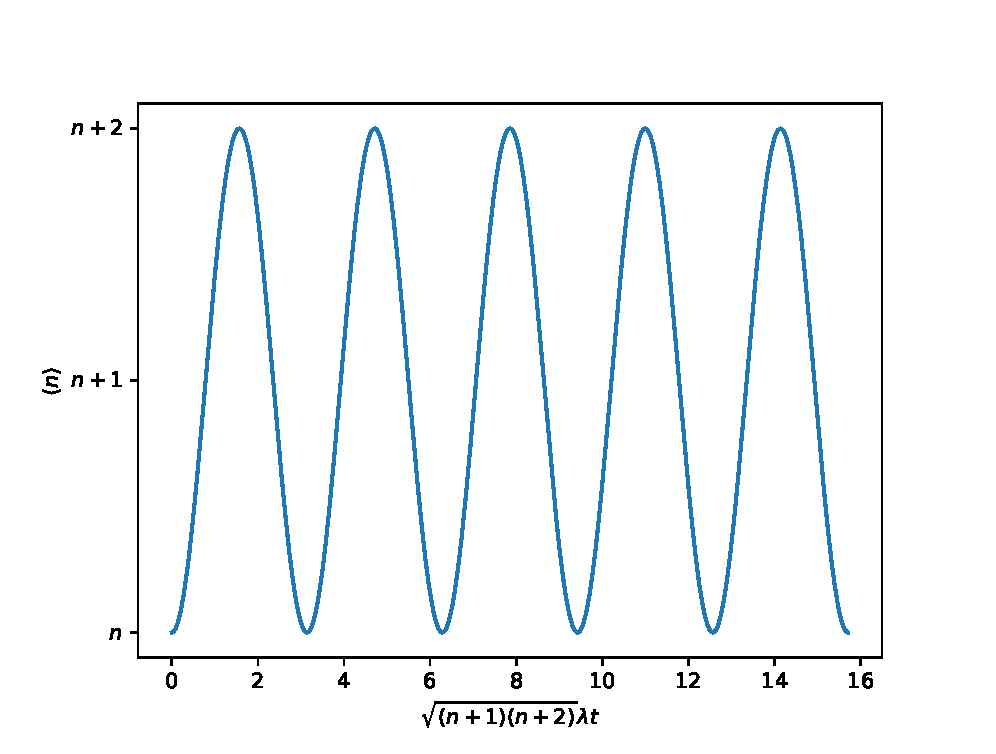
\includegraphics[width=.5\columnwidth]{Figures/2014-7.eps}
            \caption{光子数与时间的关系.}
            \label{2014-7}
        \end{figure}
    \end{itemize}
\end{sol}

\begin{prob}
    二能级原子与单模光场发生共振作用, 系统的哈密顿量为 $H=\hbar\lambda(\sigma_-a^{\dagger}+\sigma_+a)$. 如果原子 $t=0$ 时刻处于激发态 $\lvert e\rangle$, 而光场处于相干态 $\lvert\alpha\rangle$, 计算任意时刻 $t$ 原子处于基态 $\lvert g\rangle$ 的概率 $P_g(t)$, 并作出图形 (横坐标表示时间, 纵坐标为概率. 为方便, $\alpha=1$).
\end{prob}
\begin{sol}
    设系统的状态为
    \begin{align}
        \lvert\varphi(t)\rangle_{AF}=\sum_{n=0}^{\infty}[C_{e,n}\lvert e,n\rangle+C_{g,n}\lvert g,n\rangle].
    \end{align}
    相互作用绘景下, 系统的状态演化遵循薛定谔方程:
    \begin{align}
        i\hbar\frac{\partial}{\partial t}\lvert\varphi(t)\rangle_{AF}=H\lvert\varphi(t)\rangle_{AF},
    \end{align}
    即
    \begin{align}
        \dot{C}_{e,n}(t)=&-i\lambda\sqrt{(n+1)(n+2)}C_{g,n+2}(t),\\
        \dot{C}_{g,n+2}(t)=&-i\lambda\sqrt{(n+1)(n+2)}C_{e,n}(t),
    \end{align}
    解得对于 $n\in\mathbb{Z}^+$,
    \begin{align}
        C_{e,n}(t)=&C_{e,n}(0)\cos[\sqrt{(n+1)(n+2)}\lambda t]-iC_{g,n+2}\sin[\sqrt{(n+1)(n+2)}\lambda t],\\
        C_{g,n+2}(t)=&C_{g,n+2}(0)\cos[\sqrt{(n+1)(n+2)}\lambda t]-iC_{e,n}(0)\sin[\sqrt{(n+1)(n+2)}\lambda t],
    \end{align}
    此外,
    \begin{align}
        C_{g,0}(t)=&C_{g,0}(0),\\
        C_{g,1}(t)=&C_{g,1}(0).
    \end{align}
    原子初态为激发态 $\lvert g\rangle$, 光场初态为相干态 $\lvert\alpha\rangle=e^{-\abs{\alpha}^2/2}\sum_{n=0}^{\infty}\frac{\alpha^n}{\sqrt{n!}}\lvert n\rangle$, 即 $C_{g,n}=e^{-\abs{\alpha}^2/2}\frac{\alpha^n}{\sqrt{n!}}$, 将其代数上面四式中得对 $n\in\mathbb{Z}^+$,
    \begin{align}
        C_{e,n}=-ie^{-\abs{\alpha}^2/2}\frac{\alpha^{n+2}}{\sqrt{(n+2)!}}\sin[\sqrt{(n+1)(n+2)}\lambda t],\\
        C_{g,n+2}=e^{-\abs{\alpha}^2/2}\frac{\alpha^{n+2}}{\sqrt{(n+2)!}}\cos[\sqrt{(n+1)(n+2)}\lambda t],
    \end{align}
    此外,
    \begin{align}
        C_{g,0}(t)=&e^{-\abs{\alpha}^2/2},\\
        C_{g,1}(t)=&e^{-\abs{\alpha}^2/2}\alpha.
    \end{align}
    若取 $\alpha=1$, 则任意时刻 $t$ 原子处于基态的概率为
    \begin{align}
        P_g(t)=\sum_{n=0}^{\infty}\abs{C_{g,n}(t)}^2=e^{-1}\left[2+\sum_{n=2}^{\infty}\frac{\cos^2[\sqrt{n(n-1)}\lambda t]}{n!}\right],
    \end{align}
    如图 \ref{2014-8} 所示.
    \begin{figure}[H]
        \centering
        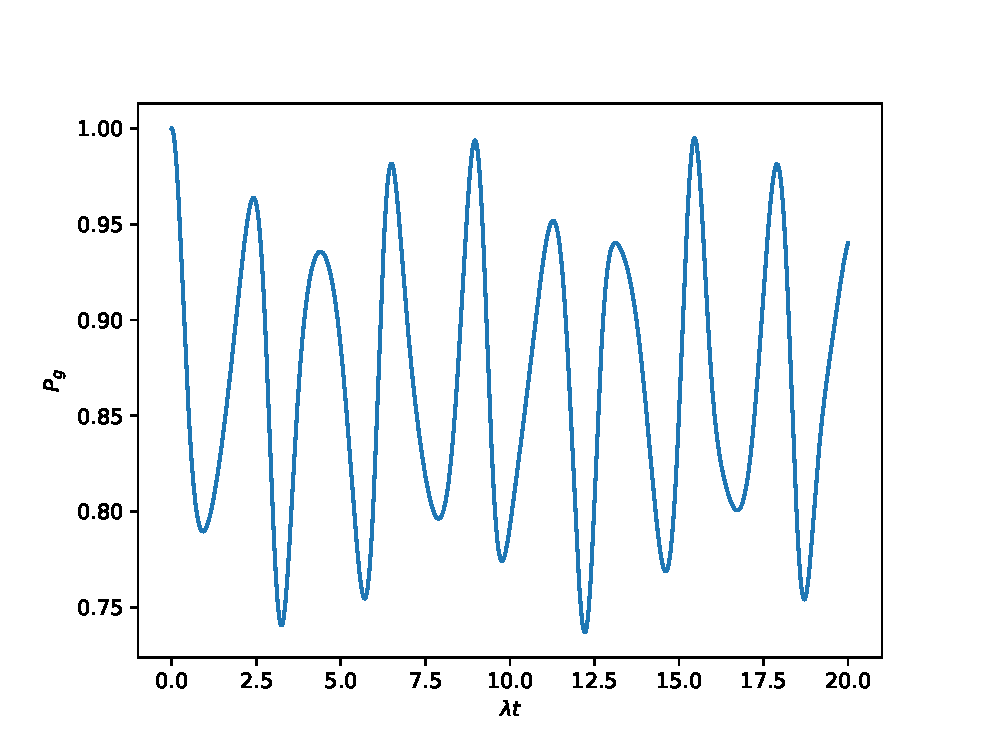
\includegraphics[width=.5\columnwidth]{Figures/2014-8.eps}
        \caption{任意时刻 $t$ 原子处于基态的概率.}
        \label{2014-8}
    \end{figure}
\end{sol}

\begin{prob}
    二能级原子与单模光场发生双光子共振相互作用, 系统的哈密顿量为 $H=\hbar\lambda[\sigma_-(a^{\dagger})^2+\sigma_+a^2]$. 假设原子初态 ($t=0$ 时刻的量子态) 为激发态 $\lvert e\rangle$, 光场初态为相干态 $\lvert\alpha\rangle$. 求系统任意时刻的量子态.
\end{prob}
\begin{sol}
    设系统的状态为
    \begin{align}
        \lvert\varphi(t)\rangle_{AF}=\sum_{n=0}^{\infty}[C_{e,n}\lvert e,n\rangle+C_{g,n}\lvert g,n\rangle].
    \end{align}
    相互作用绘景下, 系统的状态演化遵循薛定谔方程:
    \begin{align}
        i\hbar\frac{\partial}{\partial t}\lvert\varphi(t)\rangle_{AF}=H\lvert\varphi(t)\rangle_{AF},
    \end{align}
    即
    \begin{align}
        \dot{C}_{e,n}(t)=&-i\lambda\sqrt{(n+1)(n+2)}C_{g,n+2}(t),\\
        \dot{C}_{g,n+2}(t)=&-i\lambda\sqrt{(n+1)(n+2)}C_{e,n}(t),
    \end{align}
    解得对于 $n\in\mathbb{Z}^+$,
    \begin{align}
        C_{e,n}(t)=&C_{e,n}(0)\cos[\sqrt{(n+1)(n+2)}\lambda t]-iC_{g,n+2}\sin[\sqrt{(n+1)(n+2)}\lambda t],\\
        C_{g,n+2}(t)=&C_{g,n+2}(0)\cos[\sqrt{(n+1)(n+2)}\lambda t]-iC_{e,n}(0)\sin[\sqrt{(n+1)(n+2)}\lambda t],
    \end{align}
    此外,
    \begin{align}
        C_{g,0}(t)=&C_{g,0}(0),\\
        C_{g,1}(t)=&C_{g,1}(0).
    \end{align}
    原子初态为激发态 $\lvert g\rangle$, 光场初态为相干态 $\lvert\alpha\rangle=e^{-\abs{\alpha}^2/2}\sum_{n=0}^{\infty}\frac{\alpha^n}{\sqrt{n!}}\lvert n\rangle$, 即 $C_{g,n}=e^{-\abs{\alpha}^2/2}\frac{\alpha^n}{\sqrt{n!}}$, 将其代数上面四式中得对 $n\in\mathbb{Z}^+$,
    \begin{align}
        C_{e,n}=-ie^{-\abs{\alpha}^2/2}\frac{\alpha^{n+2}}{\sqrt{(n+2)!}}\sin[\sqrt{(n+1)(n+2)}\lambda t],\\
        C_{g,n+2}=e^{-\abs{\alpha}^2/2}\frac{\alpha^{n+2}}{\sqrt{(n+2)!}}\cos[\sqrt{(n+1)(n+2)}\lambda t],
    \end{align}
    此外,
    \begin{align}
        C_{g,0}(t)=&e^{-\abs{\alpha}^2/2},\\
        C_{g,1}(t)=&e^{-\abs{\alpha}^2/2}\alpha.
    \end{align}
    故系统在任意时刻 $t$ 的量子态为
    \begin{align}
        \notag&\lvert\varphi(t)\rangle_{AF}\\
        =&e^{-\abs{\alpha}^2/2}\left\{\lvert g,0\rangle+\alpha\lvert g,1\rangle+\sum_{n=0}^{\infty}\frac{\alpha^{n+2}}{\sqrt{(n+2)}}\{-i\sin[\sqrt{(n+1)(n+2)}\lambda t]\lvert e,n\rangle+\cos[\sqrt{(n+1)(n+2)}\lambda t]\lvert g,n+2\rangle\}\right\}.
    \end{align}
\end{sol}

\begin{prob}
    二能级原子与单模光场发生共振相互作用, 系统的哈密顿量为 $H=\hbar\lambda(\sigma_-a^{\dagger}+\sigma_+a)$, 如果原子 $t=0$ 时刻处于 $\cos\theta\lvert e\rangle+\sin\theta\lvert g\rangle$, 而光场处于相干态 $\lvert\alpha\rangle$, 定义原子算符 $S_1=1/2(\lvert e\rangle\langle g\rvert+\lvert g\rangle\langle e\rvert)$, 求任意时刻 $t$, $S_1$ 的平均值.
\end{prob}
\begin{sol}
    
\end{sol}

\begin{prob}
    压缩态的另一种定义: $\lvert\alpha\rangle_g=D(\alpha)S(\xi)\lvert 0\rangle$. 我们学过的压缩态为 $\lvert\beta\rangle=S(\xi(\beta))\lvert 0\rangle$. 若 $\lvert\alpha\rangle_g=\lvert\beta\rangle_g$, 利用它们关于 $X_1=1/2(a+a^{\dagger})$ 和 $X_2=-i/2(a-a^{\dagger})$ 的涨落图, 求出 $\alpha$ 和 $\beta$ 的关系。
\end{prob}
\begin{sol}
    
\end{sol}

\begin{prob}
    下图椭圆表示某压缩相干态光场的两正交分量 $X_1=1/2(a+a^{\dagger})$ 和 $X_2=-i/2(a-a^{\dagger})$ 的涨落范围. 已知椭圆长轴长为 $\Delta X_2=5$, 椭圆中心坐标为 $(0,5)$
    \begin{itemize}
        \item[(1)] 若该压缩相干态 $\lvert\beta\rangle_g=S(\xi)D(\beta)\lvert 0\rangle$, 求 $\beta$, $\xi$;
        \item[(2)] 若压缩相干态 $\lvert\beta\rangle_g=D(\beta)S(\xi)\lvert 0\rangle$, 则 $\beta$, $\xi$ 又是多少?
    \end{itemize}
\end{prob}
\begin{sol}
    \begin{itemize}
        \item[(1)] 
        \item[(2)] 
    \end{itemize}
\end{sol}

\begin{prob}
    薛定谔猫态 $\lvert\psi\rangle=x[\lvert\alpha\rangle+\lvert-\alpha\rangle]$,
    \begin{itemize}
        \item[(1)] 求归一化系数 $x$,
        \item[(2)] 定义光场的两个相位正交的振幅分量 $X_1=1/2(a+a^{\dagger})$ 和 $X_2=-i/2(a-a^{\dagger})$, 讨论 $X_2$ 的压缩条件.
    \end{itemize}
\end{prob}
\begin{sol}
    \begin{itemize}
        \item[(1)] 
        \item[(2)] 
    \end{itemize}
\end{sol}
\end{document}